\chapter{函数的极限}

前两节中,我们介绍了数列极限的理论,现在我们要将“离散型的”数列极限推广到“连续型的”函数极限中.
	
	本节课的主要内容包括:
	\begin{enumerate}
		\item 函数极限的概念;
		\item 求函数极限的方法;
		\item 函数极限的存在性准则.
	\end{enumerate}	

	\section{函数极限的概念}
	\subsection{自变量$x$无限趋大时的函数极限}
	
	在数列极限中,我们称$a$为$a_n$的极限,如果当$n \to \infty$时,$a_n$与$a$的距离充分小.在函数极限中,自变量$x$无限趋大包括三种情况: 
	\begin{itemize}
		\item $x$取正值无限趋大,记作$x \to +\infty$;
		\item $x$取负值且$\left|x\right|$无限趋大,记作$x\to -\infty$;
		\item $x$即可取正值又可取负值且$\left|x\right|$无限趋大,记作$x\to \infty$.
	\end{itemize}
	下面我们以$x \to +\infty$为例来研究函数极限的概念.类比数列极限的定义,我们可以得到以下定义:
	
	\begin{definition}[ \textbf{$x \to +\infty$时的函数极限}]
		设$f:[\alpha, +\infty) \to\mathbb{R}$是任一函数$\left(\alpha \in \mathbb{R}\right)$.如果存在常数$a$,满足:对于任意给定的正数$\varepsilon$,总存在正数$X$,使得当$x$满足$x>X$时,
		\[
		\left|f(x)-a\right|<\varepsilon,
		\]
		那么常数$a$就叫做函数$f(x)$当$x\to +\infty $时的$f(x)$的\textbf{极限},记作
		\[
		\lim_{x\to +\infty}f(x)=a.
		\]\\
		此时,称当$x\to +\infty$时,$f(x)$\textbf{极限存在}.
	\end{definition}

	也就是说,对于充分大的$x,f(x)$总能落在$a$的$\varepsilon$邻域内.下图\ref{limfun}可以从几何直观上帮助理解函数极限的定义。
	\begin{figure}[H]
		\centering
		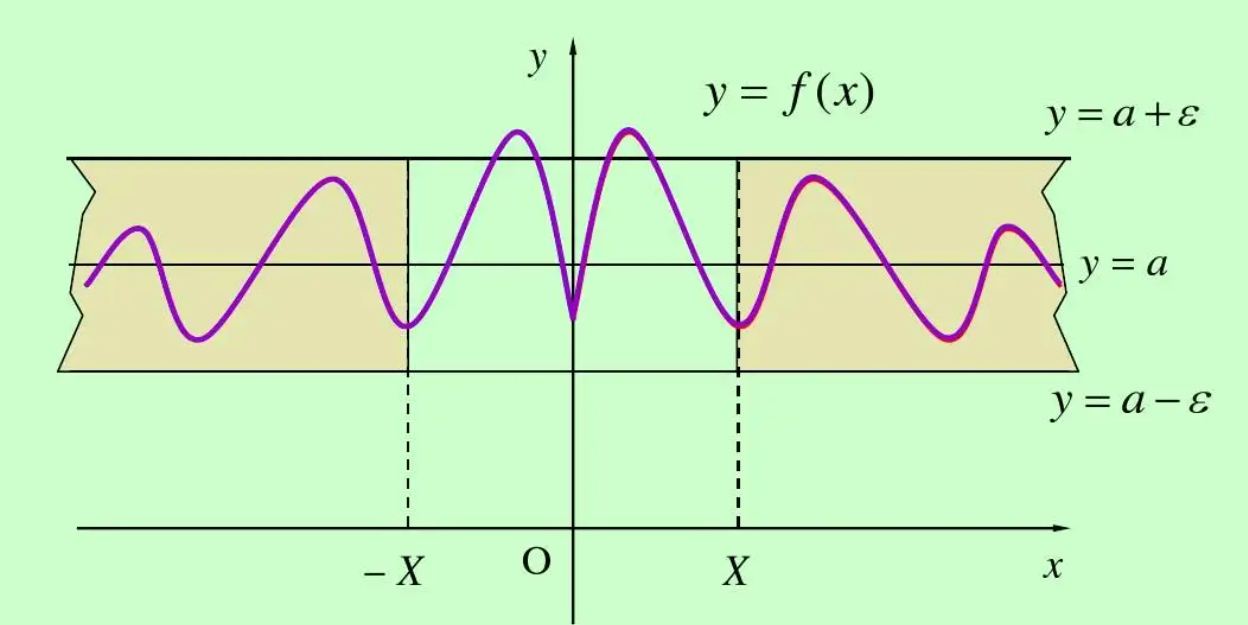
\includegraphics[width=0.7\textwidth]{figures/limfun}
		\caption{函数极限定义}\label{limfun}
	\end{figure}
	
	
	\subsection{自变量$x$趋于有限值时函数的极限}
	数列极限只研究了当自变量趋于无穷大时的极限,但是对于函数极限来说,考虑到其“连续型”的特征,我们还需要研究自变量$x$趋于有限值$x_0$时的函数极限。例如,函数连续性和导数都是用某一点处的函数极限来定义的。
	
	$x$趋于$x_0$也包括三种情形:
	\begin{itemize}
		\item 在数轴上$x$从$x_0$右侧趋近于$x_0$,记作$x \to x_{0}^{+}$;
		\item 在数轴上$x$从$x_0$左侧趋近于$x_0$,记作$x \to x_{0}^{-}$;
		\item 在数轴上$x$从$x_0$左右两侧趋近于$x_0$,记作$x \to x_{0}$.
	\end{itemize}

	下面主要讨论$x \to x_{0}$时的情况.
	
	我们需要关心当$x \to x_{0}$时,函数值$f(x)$的变化趋势.类似地,我们给出以下定义:
	\begin{definition}[\textbf{$x\to x_0$时的函数极限}]
		设函数$f(x)$在点$x_0$的某一去心邻域内有定义.如果存在常数a,对于任意给定的正数$\varepsilon$,总存在正数$\delta$,使得当x满足$0<\left|x-x_0\right|<\delta$时,
		\[
		\left|f(x)-a\right|<\varepsilon,
		\]
		那么常数a就叫做函数$f(x)$当$x\to x_0$时的$f(x)$的\textbf{极限},记作
		\[
		\lim_{x\to x_0}f(x)=a.
		\]\\
		此时,称当$x\to x_0$时,$f(x)$\textbf{极限存在}.
		
		$\star$注意x是在$x_0$的\textbf{去心邻域},不能取到$x_0$这个点.
		\
		
	\end{definition}
	
	\begin{example}
			\[
		f(x) =
		\begin{cases}
			x^2 &  x\ne 0 ,\\
			1 &  x =0 .
		\end{cases}
		\]
		在$x=0$处的函数极限为0,而不是1.
	\end{example}
	
	类似地,可以定义当$x \to x_{0}^{+}$或$x \to x_{0}^{-}$时函数的极限,分别叫做\textbf{左极限}或\textbf{右极限}.
	
	我们有如下结论:
	\[
	\lim_{x\to x_0}f(x)=a \text{当且仅当} \lim_{x\to x_{0}^{+}}f(x)=\lim_{x\to x_{0}^{-}}f(x)=a.
	\]
	也就是说,$f(x)$极限存在的充要条件是$f(x)$的左右极限都存在且相等.这个结论可以作为判断函数极限是否存在的一个方法.
	\begin{example}
		判断函数$f(x)=\frac{\left|x\right|}{x},$当$x\to 0$时极限是否存在.
	\end{example}
	\begin{solution}
		由于
		\[
		\lim_{x\to 0^-}=\lim_{x\to 0^-}\frac{-x}{x}=-1,
		\]\[
		\lim_{x\to 0^+}=\lim_{x\to 0^+}\frac{x}{x}=1,
		\]
		故左极限不等于右极限,极限不存在.
	\end{solution}

	\begin{example}
		判断函数$f(x)=e^\frac{1}{x-2}$,当$x\to 2$时极限是否存在.
	\end{example}
	\begin{solution}
		由于\[
		\lim_{x\to 2^-}f(x)=0,
		\]\[
		\lim_{x\to 2^+}f(x)=+\infty,
		\]
		故左右极限不相等,极限不存在.
	\end{solution}
	
	
	\subsection{函数极限的归并原理}
	上一节我们已经了解了数列极限的归并原理,它是连接数列和其子列极限的桥梁.下面我们将介绍函数极限的归并原理,它是连接函数极限和数列极限的桥梁.被称为\textbf{Heine定理}.
	\begin{theorem}[\textbf{Heine定理}]
		函数$f$在$x_0$处有极限a的充分必要条件是:对于任意一个收敛于$x_0$的数列${x_n}(x_n\neq x_0)$,数列${f(x_n)}$有极限a.\\
		$\star$注意$x_n\neq x_0$.
	\end{theorem}
	Heine定理有以下两个主要作用:
		\begin{itemize}
		\item 判断函数极限是否存在;
		\item 将未知的函数问题转化为已知的数列问题.
	\end{itemize}
	下面这个例题将展示Heine定理如何处理判断极限是否存在的问题.
	\begin{example}
		设$f(x)=\sin\frac{1}{x}$,证明当$x\to 0$时极限不存在.
	\end{example}
	\begin{proof}
		设$x_n=(2n\pi + \frac{\pi}{2})^{-1},y_n=(2n\pi - \frac{\pi}{2})^{-1}$,
		
		则$x_n\to 0,y_n\to 0,x_n,y_n\in ,\mathbb{R}\setminus \{0\}$,
		
		且对任意正整数$n$都有$f(x_n)=1,f(y_n)=-1,f(x_n)\ne f(y_n)$.
		
		故$f(x)$极限不存在.
	\end{proof}
	关于反三角函数,还有两个重要极限:
	\begin{example}
		$\lim\limits_{x\to +\infty} \arctan x=\frac{\pi}{2}$
		
		$\lim\limits_{x\to -\infty} \arctan x=-\frac{\pi}{2}$
	\end{example}
	
	\section{函数极限的性质}
	函数极限与数列极限有很多相似的性质,很多性质可以利用上文提到的Heine定理转化为数列极限来证明.
	
	\begin{theorem}[\textbf{唯一性}]
		设$\lim\limits_{x\to x_0}f(x)=a$,则当$x\to x_0$时,$f(x)$的极限是唯一的.
	\end{theorem}
	
	\begin{theorem}[\textbf{局部有界性}]
		设$\lim\limits_{x\to x_0}f(x)=a$,则$f$在$x_0$处是\textbf{局部有界的},即存在$M>0$与$\delta >0$,使得对于任意的$x\in \left(x_0-\delta,x_0+\delta \right)\backslash \{x_0\}$,都有$\left|f(x)\right| \le M$.
	\end{theorem}

	\begin{theorem}[\textbf{局部保号性}]
		设$\lim\limits_{x\to x_0}f(x)=a$,$\lim\limits_{x\to x_0}g(x)=b$,若$a\ne 0$,则存在$\delta >0$,使得对于任意的$x\in \left(x_0-\delta,x_0+\delta \right)\backslash \{x_0\},f(x)$都与$a$同号.特别若$a>0\left(a<0 \right),$则存在$\delta >0,$使得任意$x\in \left(x_0-\delta,x_0+\delta \right)\backslash \{x_0\}$,恒有$f(x)\ge q \ge 0\left(f(x) \le q \le 0\right)$.
	\end{theorem}

	\begin{theorem}[\textbf{局部保序性}]
		设$\lim\limits_{x\to x_0}f(x)=a$,$\lim\limits_{x\to x_0}g(x)=b$,若存在$\delta>0,$使得对于任意的$x\in \left(x_0-\delta,x_0+\delta \right)\backslash \{x_0\}$,恒有$f(x)\le g(x)$,则$a\le b$.
	\end{theorem}	
	以上三个性质都是\textbf{局部}的性质,反映函数在某一个点附近的性质.
	
	\begin{theorem}[\textbf{夹逼性}]
		设$\lim\limits_{x\to x_0}f(x)=a$,$\lim\limits_{x\to x_0}g(x)=b$,若存在$\delta>0,$使得对于任意的$x\in \left(x_0-\delta,x_0+\delta \right)\backslash \{x_0\}$,恒有$f(x) \le \phi(x) \le g(x),$且$a=b$,则$\lim\limits_{x\to x_0}\phi (x)=a$.
	\end{theorem}
	$\star$ 夹逼性定理常用于计算某些函数极限.
	\begin{example}
		计算$\lim\limits_{x\to 0}x\left[\frac{1}{x}\right]=1$.
	\end{example}
	\begin{solution}
		由于$x(\frac{1}{x}-1)\le x\left[\frac{1}{x}\right]\le x\cdot \frac{1}{x}$,
		
		且$\lim\limits_{x\to 0}x(\frac{1}{x}-1)=1,\lim\limits_{x\to 0}x\cdot \frac{1}{x}=1$,
		
		故$\lim\limits_{x\to 0}x\left[\frac{1}{x}\right]=1$.
	\end{solution}
	
	\begin{theorem}[\textbf{有理运算法则}]
		设$\lim\limits_{x\to x_0}f(x)=a$,$\lim\limits_{x\to x_0}g(x)=b$,则
		\begin{enumerate}
			\item 
			\[\lim_{x\to x_0}(f(x)\pm g(x))=\lim_{x\to x_0}f(x) \pm \lim_{x\to x_0}g(x)=a\pm b;
			\]
			\item 
			\[\lim_{x\to x_0}f(x)g(x)=\lim_{x\to x_0}f(x) \lim_{x\to x_0}g(x)=ab;
			\]
			\item 
			\[\lim_{x\to x_0}\frac{f(x)}{g(x)}=\frac{\lim\limits_{x\to x_0}f(x)}{\lim\limits_{x\to x_0}g(x)}=\frac{a}{b},\text{其中}b \ne 0.
			\]
		\end{enumerate}
	\end{theorem}
	以上几个定理同样适用于$x\to \infty,x \to \pm\infty, x\to x_{0}^{\pm}$等情形.
	\begin{example}
		若$\lim\limits_{x\to x_0}f(x)$和$\lim\limits_{x\to x_0}(f(x)-g(x))$都存在,则$\lim\limits_{x\to x_0}g(x)$也存在.
	\end{example}
	
	\begin{theorem}[\textbf{复合函数极限运算法则}]
		设$y=(f\circ g)(x)=f(g(x))$是由$y=f(u)$与$u=g(x)$复合而成,复合函数$f\circ  g$定义在$x_0$的某去心邻域$\overset{\circ}{U}(x_0)$中.若$\lim\limits_{x\to x_0}g(x)=u_0,\lim\limits_{u\to u_0}f(u)=a,$并且存在$\delta _0>0$,使得对于任意的$x\in \overset{\circ}{U}(x_0,\delta_0),$恒有$g(x)\ne u_0$,则
		\[\lim_{x\to x_0}f(g(x))=a=\lim_{u\to u_0}f(u).
		\]
	\end{theorem}	
	此定理给出了求复合函数极限时,运用变量替换法的条件.复合函数极限运算法则可以应用于下一个部分,之后将给出例题.	
		

	\section{两个重要极限}
	下面介绍两个非常重要且常用的极限,它们不仅可以用来求复杂函数的极限,也是推导导数公式的基础.
	\begin{enumerate}
		\item 	$\lim\limits_{x\to 0}\frac{\sin x}{x}=1$;
		\item 	$\lim\limits_{x\to \infty}(1+\frac{1}{x})^x=e$.
	\end{enumerate}
	这两个极限的证明见教材,请同学们尽量掌握.
	
	\begin{example}
		求$\lim\limits_{x\to 0}\frac{\sin2x}{x}.$
	\end{example}
	\begin{solution}
		\[
		\lim\limits_{x\to 0}\frac{\sin2x}{x}=\lim\limits_{x\to 0}\frac{\sin2x}{2x}\cdot 2=2\].
	\end{solution}

	\begin{example}
		求$\lim\limits_{x\to 0}x\cot 2x$.
	\end{example}
	\begin{solution}
		\[
		\lim\limits_{x\to 0}x\cot 2x=\lim\limits_{x\to 0}x\cdot\frac{\cos 2x}{\sin 2x}=\lim\limits_{x\to 0}\frac{2x}{\sin2x}\cdot\frac{\cos2x}{2}=\frac{1}{2}.
		\]
	\end{solution}

	\begin{example}
		求$\lim\limits_{x\to 0}(1-3x)^{\frac{2}{x}}.$
	\end{example}
	\begin{solution}
		\[
		\lim\limits_{x\to 0}(1-3x)^{\frac{2}{x}}=\lim\limits_{x\to 0}(1+(-3x))^{-\frac{1}{3x} \cdot (-3x) \cdot \frac{2}{x}}=e^{\lim\limits_{x\to 0}-\frac{6x}{x}}=e^{-6}. 
		\]
	\end{solution}

	\begin{example}
		求$\lim\limits_{x\to 0}(\cos x+x\sin x)^{\frac{1}{x^2}}.$
	\end{example}
	\begin{solution}
		\begin{align*}
		\lim\limits_{x\to 0}(\cos x+x\sin x)^{\frac{1}{x^2}}&=\lim\limits_{x\to 0}(1+\cos x+x\sin x-1)^{\frac{1}{x^2}}\\
		& = \lim\limits_{x\to 0}(1+\cos x+x\sin x-1)^{\frac{1}{\cos x+x\sin x-1}\cdot \frac{\cos x+x\sin x-1}{x^2}}\\
		& = {\rm e}^{\lim\limits_{x\to 0}\frac{\cos x+x\sin x-1}{x^2}}\\
		& = {\rm e}^{\lim\limits_{x\to 0}\frac{\cos x-1}{x^2}+\frac{\sin x}{x}}\\
		& = {\rm e}^{-\frac{1}{2}+ 1}\\
		& = {\rm e}^{\frac{1}{2}}.
		\end{align*}
	\end{solution}
	
	\section{函数极限的存在准则}
	与数列极限类似,下面将介绍函数极限的单调有界准则和Cauchy收敛原理.
	\begin{theorem}[\textbf{单调有界准则}]
		
			\begin{enumerate}
				\item 	设函数$f$在区间$\left[a,+\infty \right) \left(a\in \mathbb{R} \right)$上单调增或减,有上或下界,则$\lim\limits_{x\to x_0}f(x)$存在;
				\item 	设函数$f$是区间$I$上的单调函数,则$f$在$I$内每一点的单侧极限存在.
			\end{enumerate}
	\end{theorem}

	\begin{theorem}[\textbf{Cauchy收敛原理}]
		设$f:\overset{\circ}{U}(x_0)\to \mathbb{R}$是任一函数,则$\lim\limits_{x\to x_0}f(x)$存在的充要条件是:对于任意$\varepsilon>0$,存在$\delta>0$,使得对于任意的$x_1,x_2\in \overset{\circ}{U}(x_0,\delta)$,恒有
		\[
		\left|f(x_1)-f(x_2)\right|<\varepsilon,
		\]
		其中$\overset{\circ}{U}(x_0,\delta)\subseteq\overset{\circ}{U}(x_0)$.
	\end{theorem}
	几何直观上来看,若$\lim\limits_{x\to x_0}f(x)$存在,则当$x\to x_0$时,$f$的振幅趋于零.这就为我们提供一种证明函数极限不存在的新思路.
	
	例如,函数$f(x)=\sin\frac{1}{x}$的图像(如图\ref{sinfun})在$x=0$附近不停振荡,不满足Cauchy收敛原理,因此它在$x=0$处的极限不存在.
	\begin{figure}[H]
		\centering
		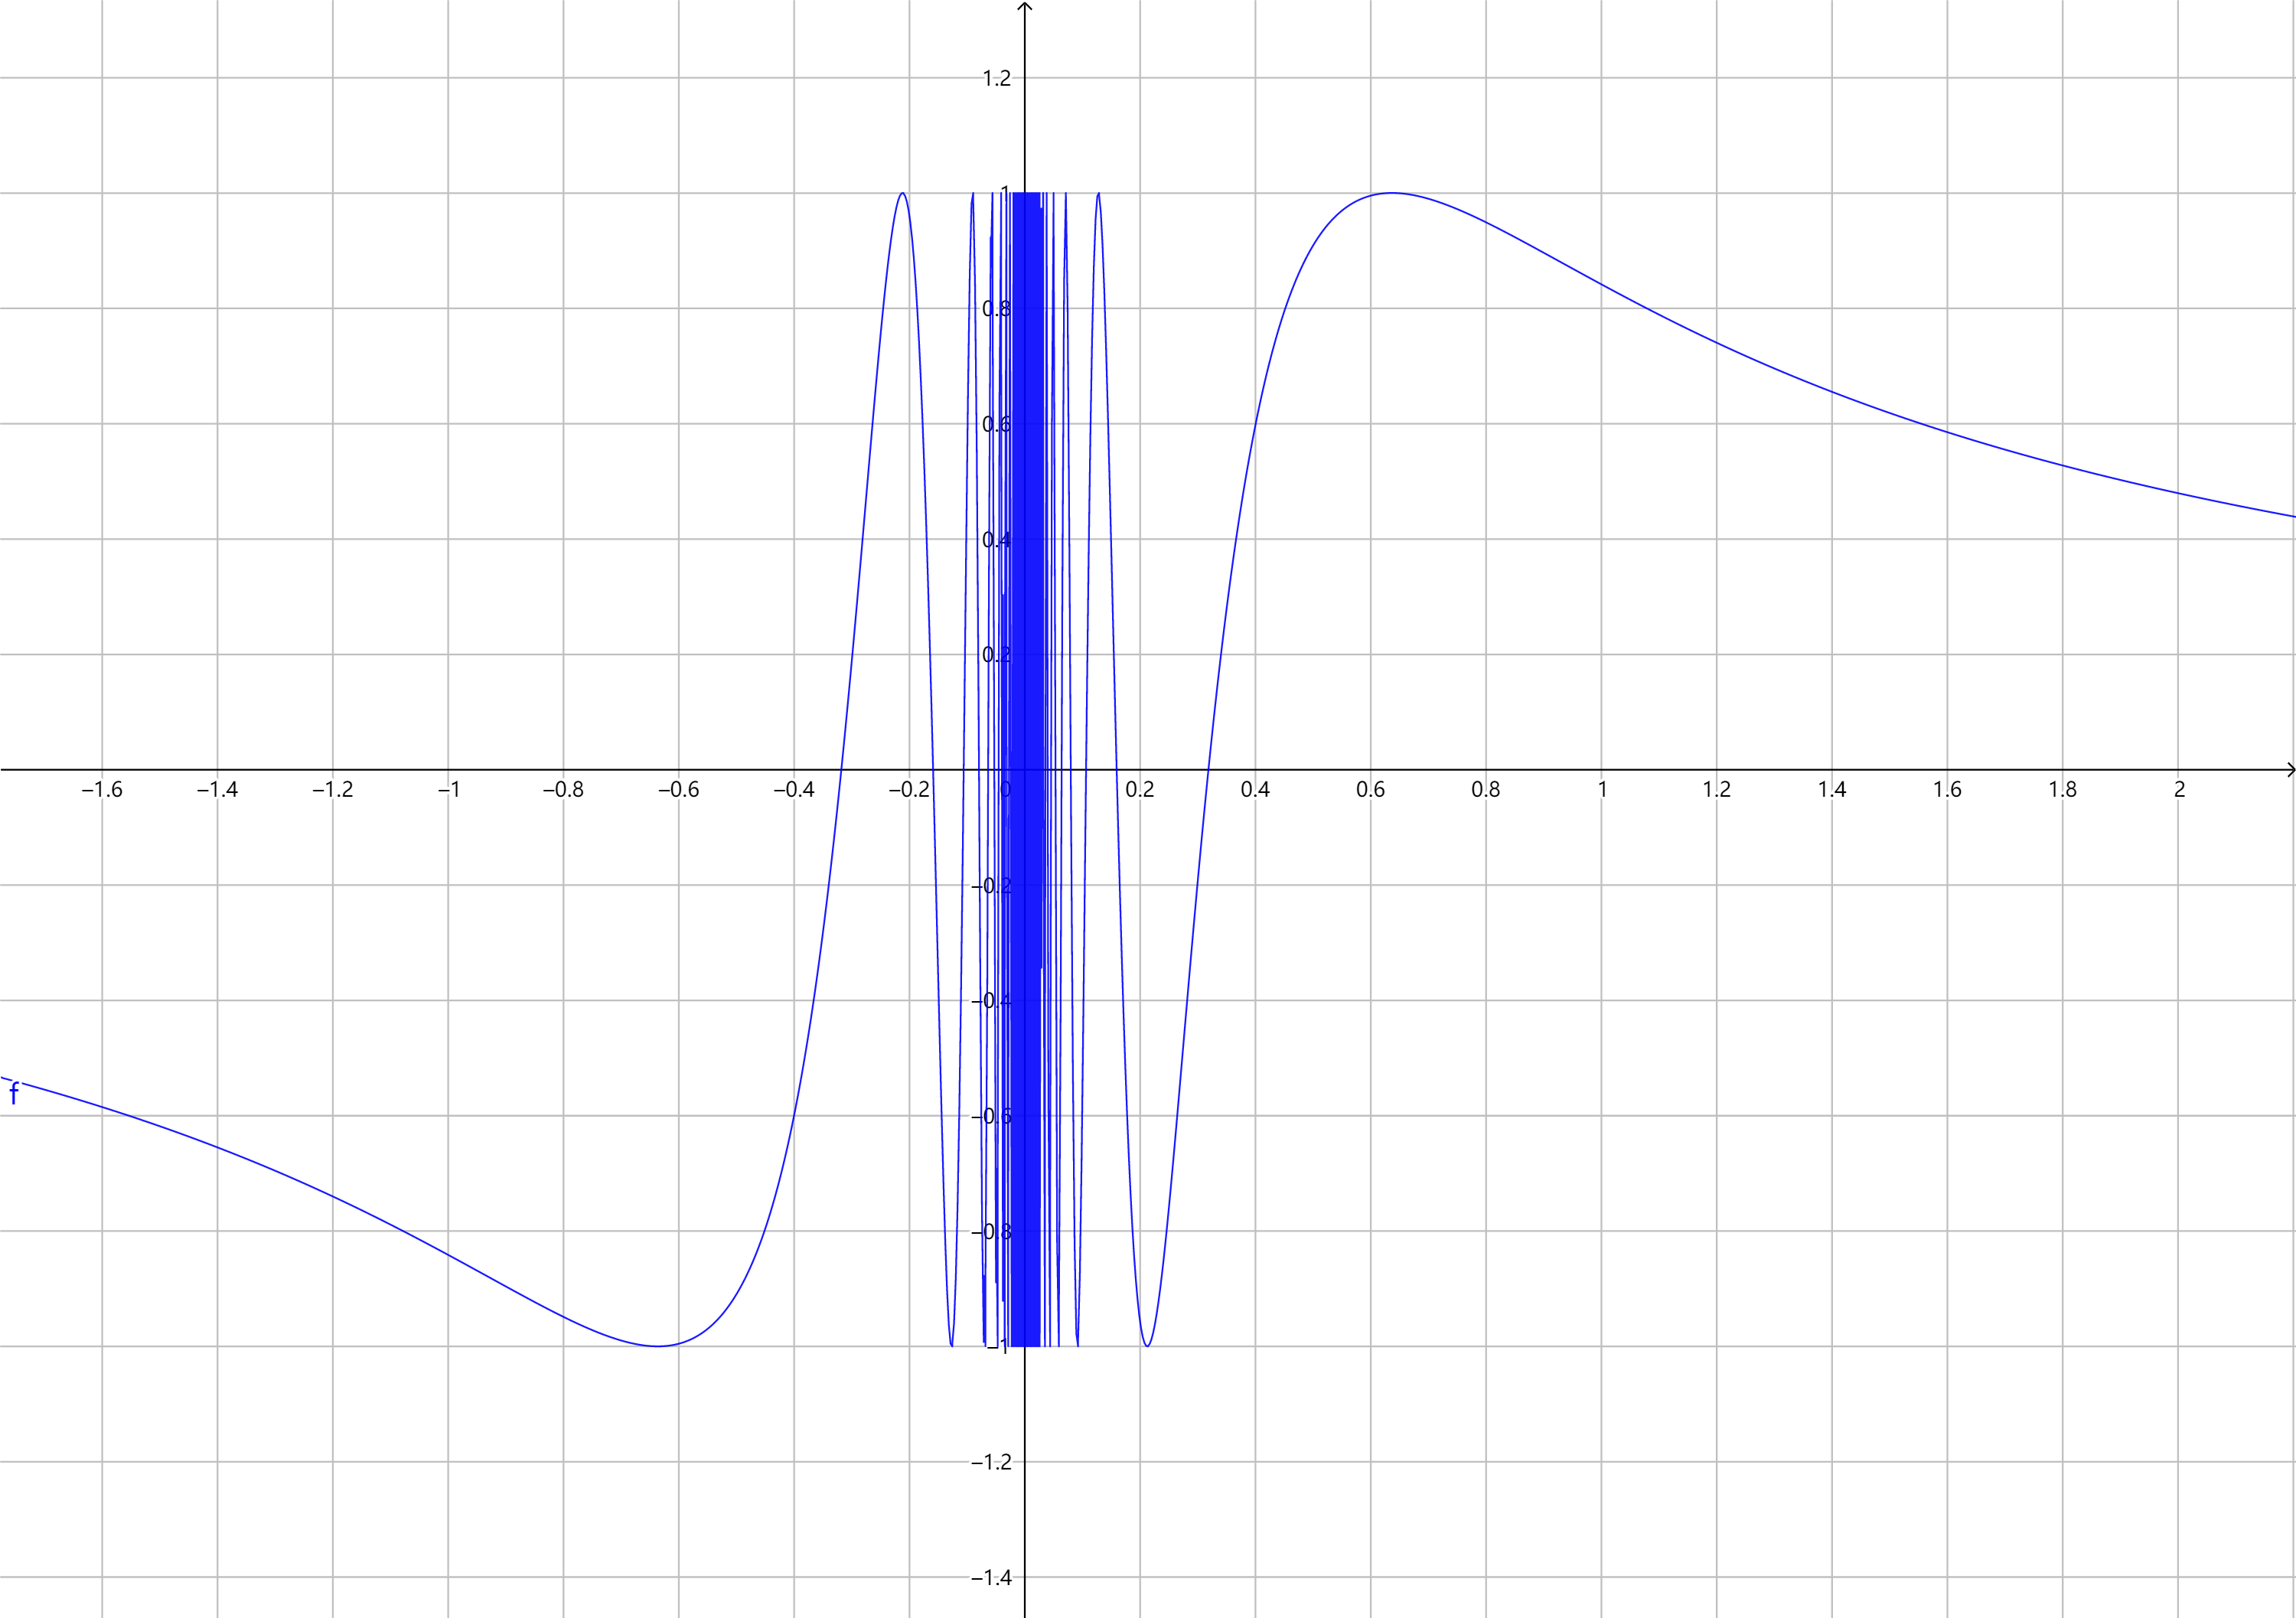
\includegraphics[width=0.5\textwidth]{figures/sinfun}
		\caption{$f(x)=\sin\frac{1}{x}$图像}\label{sinfun}
	\end{figure}